\documentclass{article}

\title{Aulas de Redes Neurais - 2018/1}

\usepackage{Sweave}
\begin{document}
\Sconcordance{concordance:02.tex:02.Rnw:%
1 4 1 1 0 6 1 1 2 1 0 1 3 1 0 1 1 1 3 1 0 1 1 1 3 1 0 1 1 1 3 1 0 1 3 1 %
0 1 1 3 2 2 1 5 0 1 3 1 1}


\maketitle

\section{Aula 09/03/2018}

\begin{Schunk}
\begin{Sinput}
> rm(list=ls())
> # parametro da gaussiana
> r1<-1.20
> r2<-1.20
> # centro da gaussiana
> m1<-pi/2
> m2<-3*pi/2
> # pesos
> w1<-1
> w2<--1
> # entradas
> u<-seq(0,2*pi,0.01)
> # funcoes intermediarias
> h1<-exp(-((u-m1)^2)/r1^2)
> h2<-exp(-((u-m2)^2)/r2^2)
> fg<-sin(u)
> yhat<-h1*w1+h2*w2
> plot(u,fg,type='l',col='black',xlim=c(0,2*pi),ylim=c(-1,1))
> par(new=T)
> plot(u,yhat,type='l',col='red',xlim=c(0,2*pi),ylim=c(-1,1))
> 
\end{Sinput}
\end{Schunk}
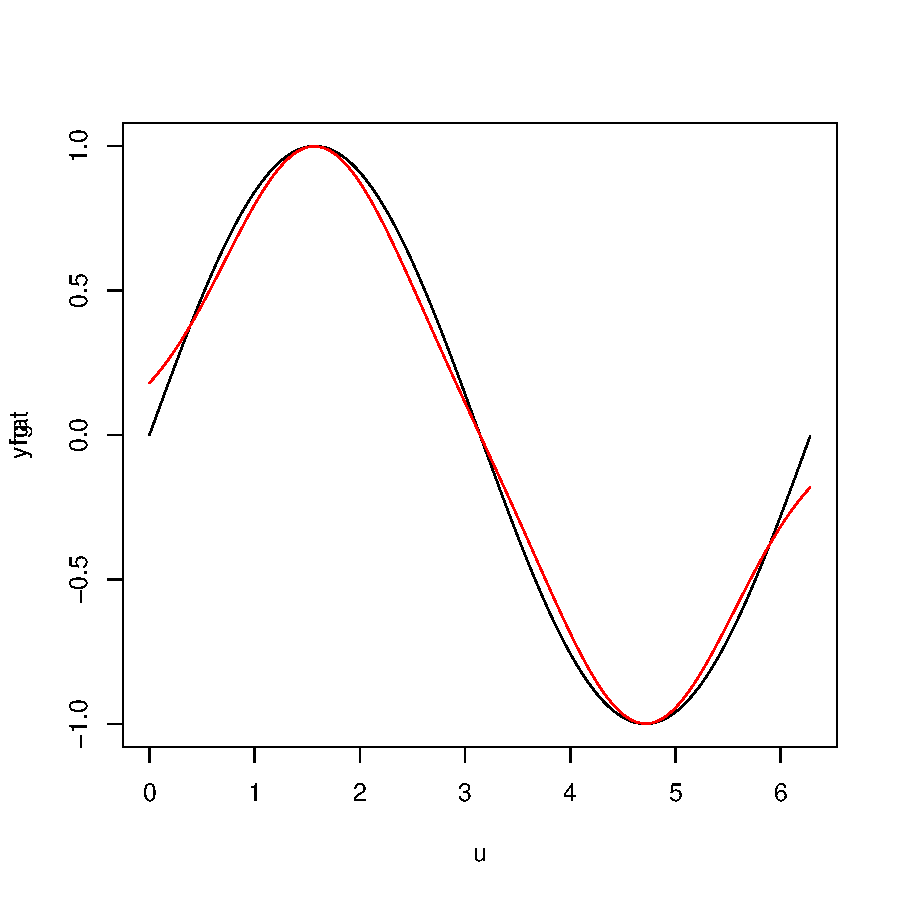
\includegraphics{02-001}

\end{document}
